
\subsection{Models}

This section will cover the main theoretical aspects of the project and give a
general description of the mathematical principles behind the machine learning
models used in this project. It will also describe the different configurations
for our experiments and models, aswell as it will motivate the use of Polyglot
embeddings.


\subsubsection{General structure of the models}

We used two different models to run our experiments. The base structure of the
models are inspired by the models used by other authors on similar
tasks~\cite{huang2015bidirectional}, ~\cite{plank2016multilingual},
~\cite{reimers2017reporting}, ~\cite{ma2016endtoend}. The first one is a
standard bidirectional LSTM network, \texttt{Bi-LSTM}, and the second one is a
\texttt{Bi-LSTM} with an added CRF layer, \texttt{Bi-LSTM-CRF} (LSTMs and CRFs
are described in greater details in Section~\ref{sec:setup-models-lstm}
and~\ref{sec:setup-models-crf} respectively). Both models has the same
fundamental structure, which consist of:

\begin{itemize}
    \item An embedding layer with a fixed embedding dimension size
    \item A dropout layer with a dropout rate of $0.5$
    \item Two LSTM layers, one for the forward pass and one for the backward
        pass\footnote{The DyNet implementation actually uses 4 LSTM layers, as
            it has 2 bidirectional LSTM layers. See
        Section~\ref{sec:setup-implementations-dynet} for more}
    \item Another dropout layer with the same dropout rate
    \item A simple linear layer mapping the LSTM output scores back into tag
        space
\end{itemize}

In the \texttt{Bi-LSTM} model, the output of the final linear layer is run
through a softmax activation function. In the \texttt{Bi-LSTM-CRF} model, the
output is instead treated as emission scores that is passed as input to the CRF
layer, which then compute the most likely sequence of tags.

The size of the embedding layer is $100004 \times 64$, meaning it has an input
size of 100004 and produces an output vector of size 64. The size of each LSTM
layer is $64 \times 100$, and since the output of each LSTM is concatenated, we
get a 200 dimensional output. The size of the simple linear layer is 200 x
number of tags, depending on the task. With CRF the last layer contains 2
additional tags because of an implementation detail.

By simple linear layer we mean a layer which takes an input vector $x$ and makes
a linear transformation on the input using a weight matrix $W$ and a bias vector
$b$. The input vector is then transformed as follows $W \cdot x + b$. Where $W
\cdot x$ is a matrix vector multiplication, meaning the vector is treated as a
matrix with dimensions $n,1$ and standard matrix multiplication is used,
producing a new vector with the same size as the numer of rows in the weight
matrix.

For training we use the stochastic gradient descent (SGD) optimizer since it
seems to give the best results, but with slower convergence during
training~\cite{yang2018design}. We use a learning rate of 0.1 and no weight
decay or momentum.

The loss function for the softmax model is the negative log likelihood of the
correct tag. 

\subsubsection{Embeddings}

We use a pretrained embedding since they have been shown to provide a
significant increase in accuracy for sequence labeling tasks
(~\cite{yang2018design}). We picked pretrained Polyglot
embeddings~\cite{polyglot:2013:ACL-CoNLL} since there exists models in a lot of
different languages, and Polyglot seems to outperform the only alternative we
were aware of FastText~\cite{joulin2016bagoftricks} (~\cite{plank2018distant} to
FastText + comparison), even though FastText embeddings are significantly larger
than Polyglot's. There exists many different algorithms for training word
embeddings, but not many with trained models in a wide range of languages
available. Polyglot contains vector representations for 100.000 different words,
as well as 4 special tokens. Each vector representation has a size of 64.

The use of word embeddings can be considered a case of multi-task learning.
Multi-task learning is where multiple tasks are solved to improve the prediction
accuracy. The different tasks would let the model learn some shared structure
between the two tasks which allows for better generalization. This is a
regularization technique which works well because it introduces more data for
the models to train on as well as prevent the model from overfitting on one
task~\cite{goodfellow2016deep}. 

For our case, the word embedding is trained on one set of data to learn
representations of words, where similar words have similar representations.
Afterwards the word embedding as well as the rest of the model is trained on a
new task where the model learns task specific representations. But since the
word embeddings start from a useful initial configuration it is unlikely to
forget much of the previous representation and is therefore better able to
generalize.

Another way to think about the word embedding is as a linear layer where the
input is a one-hot vector representation of the word~\cite{goldberg2017nerual}.
A one-hot vector is a vector where all but a single value in the vector are zero
and the element corresponding to a word is one. Similar to word embeddings where
we lookup a word and return a vector representation, the matrix-vector
multiplication of the one-hot vector and the linear layer matrix would return a
row from the matrix, which can be considered the representation of the word. The
bias vector usually found in linear layers could simply be ignored. The
difference between a word embedding and a linear layer would then for the most
parts be that word embeddings are pretrained.

\subsubsection{Bi-LSTM}\label{sec:setup-models-lstm}

Long Short-Term Memory (LSTM) networks are a particular type of Recurrent Neural
Networks (RNN), that was originally proposed by~\cite{hochreiter1997long} as a
way of dealing with deficiencies of normal RNNs. For machine learning tasks
concerned with sequential data it is more often than not necessary to let
information about an input at a timestep $t$ get carried over to the processing
of an input at timestep $t+1$. For example, when processing a sentence like
`Since Netta won the Eurovision Song Contest 2018 it will be hosted by Israel
next year', the model will only be able to know what `it' refers to, if it
remembers that the sentence is currently (ie.\ at the given time step $t$) about
`the Eurovision Song Contest 2018'. This is the motivation of RNN (see
Figure~\ref{fig:rnn}).

Standard Recurrent Neural Networks calculates two values, a hidden value, which
is used to carry information from one timestep to the next, and the output. The
values are calculated as follows (~\cite{goodfellow2016deep}):

\begin{align*}
    & \textbf{a}_t = \textbf{b} + \textbf{W} \textbf{h}_{t-1} + \textbf{U} \textbf{x}_t \\
    & \textbf{h}_t = \tanh(\textbf{a}_t) \\
    & \textbf{o}_t = \textbf{c} + \textbf{V} \textbf{h}_t \\
    & \textbf{y}_t = softmax(\textbf{o}_t)
\end{align*}

Its not much more complicated than a simple linear layer. There are two
additional matricies and an additional bias vector. The input $x_t$ is used
along with the hidden value calculated from the previous input value $x_{t-1}$,
to calculate the new hidden value. The tanh function is used to squeeze the
hidden value between 0 and 1, which will be used for the next timestep, but is
also used for the output after a linear transformation and a softmax activation.
This way the output of the layer is not just dependent on the input, but also
all the previous input values seen.

\begin{figure}[h]
    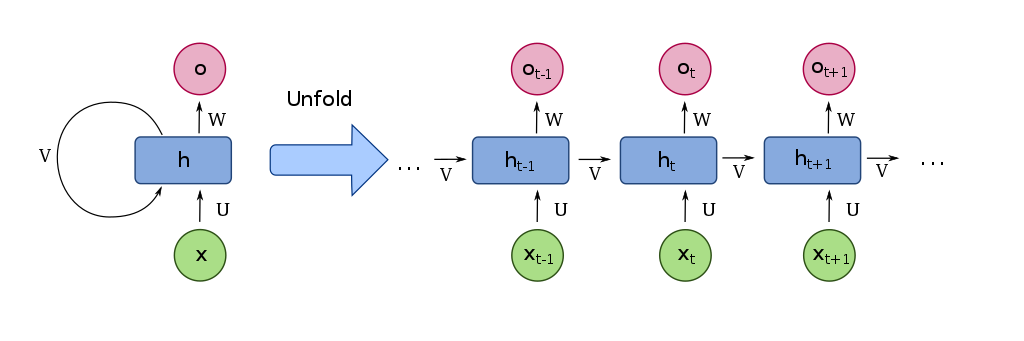
\includegraphics[width=\textwidth]{rnn-figure}
    \caption{A graphical representation of a RNN.\ The right image shows the
    model unfolded over a number of time steps. Source:~\cite{olah2015lstm}.
    }\label{fig:rnn}
\end{figure}

However, the standard RNN suffers from the problems of exponential decay or blow
up of error signals that are backpropagated through the network --- a situation
that only gets worse as the time dependencies increase
(~\cite{hochreiter2001gradient}). To remedy this, LSTM networks are used instead.

An LSTM network is composed of carefully designed memory cells containing
multiple special purpose weight matricies called gates, that determines what
information to remember, what to forget, what to do with the input and the
output of the network. In addition, a main state, $c$, of the network cell is
maintained and used to compute a hidden state, $h$, which is passed on to be
used at the next timestep, similar to the standard RNN.

The gates and states are calculated in the following manner
(~\cite{huang2015bidirectional}):\footnote{Note that
    these calculations are done by the respective frameworks we have been
working with and are not something, we have implemented ourselves}


\begin{align*}
    & i_{t} = \sigma(W_{xi}x_{t} + W_{hi}h_{t-1} + W_{ci}c_{t-1} + b_{i})    \\
    & f_{t} = \sigma(W_{xf}x_{t} + W_{hf}h_{t-1} + W_{cf}c_{t-1} + b_{f})    \\
    & o_{t} = \sigma(W_{xo}x_{t} + W_{ho}h_{t-1} + W_{co}c_{t-1} + b_{o})    \\ \\
    & c_{t} = f_{t}c_{t-1} + i_{t}\tanh(W_{xc}x_{t} + W_{hc}h_{t-1} + b_{c}) \\
    & h_{t} = o_{t}\tanh(c_{t})
\end{align*}

where $i_{t}$, $f_{t}$ and $o_{t}$ are the input gate, the forget gate and the
output gate respectively at time $t$, $c$ is the cell state and $h$ is the
hidden state. The weight matrices $W$ maps from either an input $x$ of size $m$
to an internal state or gate of size $n$ (ie. $W_{xf} \in \mathbb{R}^{m \times
n}$ is the input-forget gate matrix), or between two internal components (ie.
$W_{hi} \in \mathbb{R}^{n \times n}$ is the hidden-input gate matrix)
(~\cite{huang2015bidirectional}). A graphical representation of an LSTM Network
is given in Figure~\ref{fig:lstm}.

\begin{figure}[h]
    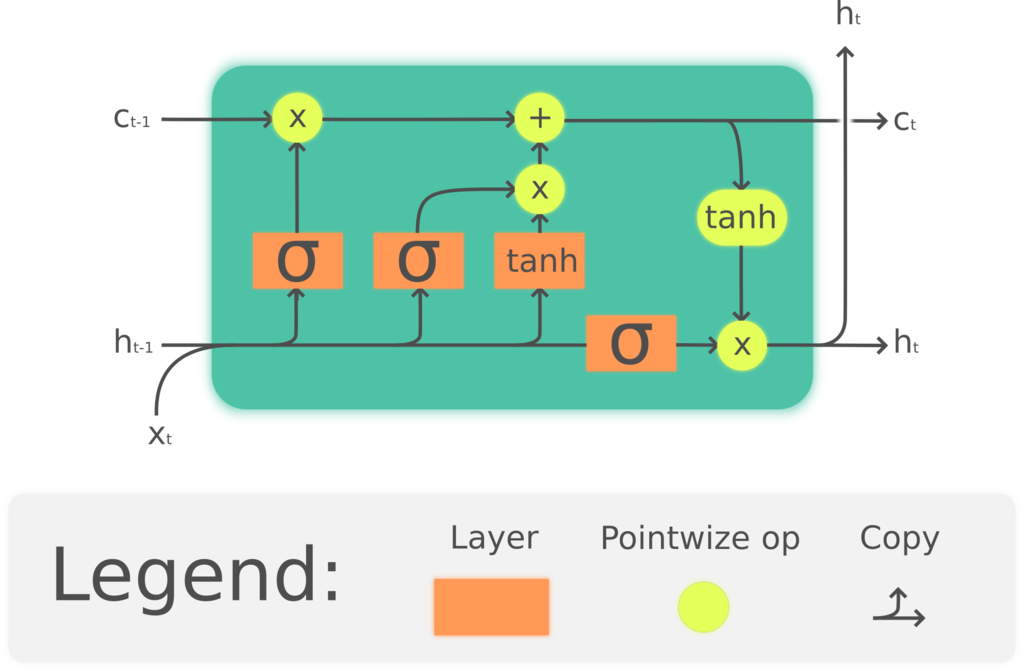
\includegraphics[width=\textwidth]{lstm-figure}
    \caption{A graphical representation of an LSTM unfolded. Source:~\cite{olah2015lstm}.
    }\label{fig:lstm}
\end{figure}

The activation function $\sigma$ is the sigmoid function, which squishes the
values of the gate matrices into the interval $[0,1]$. This means, that the
gates determine which and how much information is passed through and stored in
the memory cell. For example, the forget gate $f_{t}$ at timestep $t$ is
multiplied with the previous cell state $c_{t-1}$ to determine what to remember
and what to forget when $c_{t}$ is computed. A value of $1$ in the gate matrix
means `keep all' where a $0$ means `forget all'.\footnote{This particular forget
    mechanism was not introduced by Hochreiter in his original LSTM paper and,
    according to~\cite{pitis2016lstm}, `led the original [\ldots] model to have
    trouble with simple tasks involving long sequences'. This solution was
    introduced by~\cite{gers1999learning} and is now standard in LSTM
implementations.}

Updating the cell state also entails adding the element wise product of the
input gate $i_{t}$ and \textit{the candidate write} given by $\tanh(W_{xc}x_{t}
+ W_{hc}h_{t-1} + b_{c})$. Since the hidden state $h_{t} = o_{t}\tanh(c_{t})$
the candidate write at timestep $t$ consists of not only the weighted current
input $W_{xc}x_{t}$ but also the weighted result of passing the previous cell
state through the previous output gate $W_{hc}h_{t-1}$ where $h_{t-1} =
o_{t-1}\tanh(c_{t-1})$.

In other words, the memory cell at timestep $t-1$ produces a reading of its own
cell state which it passes on as a hidden state to the memory cell at timestep
$t$ to be used to compute the candidate write for $c_{t}$. For further
discussion of this somewhat reversed read/write procedure, refer
to~\cite{pitis2016lstm}.

The intricate design of the LSTM memory cell allows for time dependencies
spanning very long sequences through careful regulation of the cell state.
Applying a separate LSTM network layer that processes the same sequence of data
but in reversed order, the model becomes bidirectional. This means, that the
model can also use information from `the future' (ie.\ at later timesteps) to
infer knowledge about input at the current timestep.

However, at each timestep $t$ there will be two memory cells: one for the
forward pass and one for the backward pass. The first will depend on all $x_{i}
\in \{x_{0}, \ldots, x_{t-1}\}$ where the second will depend on all $x_{j} \in
\{x_{t+1}, \ldots, x_{T}\}$. This requires that the entire sequence of data is
provided before an output can be produced, but at the same time it enables the
output to be computed taking both past and future dependencies into
consideration.


\subsubsection{CRF}\label{sec:setup-models-crf}

When performing sequence labelling as we do in part-of-speech tagging and named
entity recognition, we want to predict a sequence of output tags $\bm{y} \in
\mathbb{R}^{K}$, where $K$ is the sequence length, given a sequence of input
features $\bm{X} \in \mathbb{R}^{K \times C}$ where $C$ is the number of
possible classes each tag can take.

The Conditional Random Field model (CRF) provides a method for computing the
probability of an output sequence $\bm{y}$ given an input sequence $\bm{X}$
under the assumption, that there exists conditional dependencies for
transitioning between any two $y_{k}$ and $y_{k+1}$ where $k \leq K$.

For example, in named entity recognition we work with tags such as `O', `B-PER'
and `I-PER', which classify words as non-entities (`O', eg.\ `Hello'), the first
part of a person entity (`B-PER', eg.\ `Claus') or a word inside a person entity
(`I-PER', eg.\ `Madsen'). Here, we assume that there is a higher probability of
transitioning from a tag `B-PER' to a tag `I-PER' than, say, from a tag `O' to a
tag `B-PER'.  That means, that the probability of tag $y_{k}$ being of some tag
type is conditioned on whatever $y_{k-1}$ was.

Knowing these transitioning scores, which will be the learnable parameters of
the CRF model, we can compute the conditional probability of specific sequence
of tags given an input sequence of feature vectors $p(\bm{y}|\bm{X})$.

The input sequence is often called the emission scores and that is what we will
use here onwards. The emission scores in our model comes from the feature
representation generated by the Bi-LSTM network after they have been passed
through the linear layer and mapped to tag space. 

For a regular classification problem, we could now compute $p(\bm{y}|\bm{X})$ by
taking the product of the probability of all $y_{k} \in \bm{y}$ and dividing it
by the normalization factor $Z(\bm{X}) = \prod_{k=1}^{K} Z(\bm{x}_{k})$ (also
known as the \textit{partition function}):

\begin{align*}
p(\bm{y}|\bm{X}) & = \prod_{k=1}^{K} \frac{\exp( W(\bm{x}_{k}, y_{k}) )} 
                                            {Z(\bm{x}_{k})} \\
                 & = \frac{\exp( \sum_{k=1}^{K} W(\bm{x}_k, y_{k}) )}
                                            {Z(\bm{X})}
\end{align*}

where $W(y_{k}, \bm{x}_{k})$ is the emission scores generated by the LSTM
network, here represented with a weight matrix $W$ to be consistent with general
notation (~\cite{treviso2019crf}).

For a conditional random field model however, we want to include the
dependency between label $y_{k-1}$ and $y_{k}$. This can be done by multiplying
with the probability of $y_{k}$ given $y_{k-1}$, ie. $p(y_{k}|y_{k-1})$. For
this, a transition matrix $T \in \mathbb{R}^{C \times C}$ is introduced, which 
is the trainable parameter of the CRF model:

\begin{equation*}
p(\bm{y}|\bm{X}) = \frac{\exp( \sum_{k=1}^{K} W(\bm{x}_k, y_{k}) +
                    \sum_{k=1}^{K-1} T(y_{k+1}, y_{k}) )}{Z(\bm{X})}
\end{equation*}

The challenge from here is to calculate the partition function $Z(\bm{X})$ as
this has to sum over all possible values of $y_{k}$ for all $1 \leq K$. This is
infeasable if implemented in a naive manner, but the whole crux of CRF is the
\textbf{forward} (or \textbf{backward}) algorithm, which enables the computation
to be done in time proportional to $O(CK^{2})$. A detailed description is out of
scope for this report, but is explained in great detail
in~\cite{sutton2012introduction}.

Performing inference using a CRF model (ie.\ predicting the most likely sequence
of tags $\bm{y^{*}} = \argmax_{y}p(\bm{y}|\bm{X})$) is done using the Viterbi
algorithm (~\cite{sutton2012introduction} something). This exploits the same
recursive feature of the model as the forward algorithm uncovers, and then
stores backpointers to the most likely tag $y^{*}$ at each time step $k$.

In short, our \texttt{Bi-LSTM-CRF} model is simply an extension of the
\texttt{Bi-LSTM} with an added CRF layer for modelling the conditional
dependencies between each successive tag in the sequence.

\subsubsection{Dropout layers}

The dropout layers are not part of the model besides training. Dropout is a
regularization technique which helps prevent the model from
overfitting~\cite{goodfellow2016deep}. Regularization is when we make changes to
reduce a models generalization error, ie.\ the errors on the test data, possibly
introducing more errors on the training data. Many different regularization
techniques exist and dropout is just one of these.

Dropout is about introducing variance in the model trained by randomly removing
output values. When thinking of the model as a network of neurons, dropout is
like randomly removing neurons from this network. What this means in relation to
the computational graph built, is that some of the elements in the vector output
of a node in the graph, is set to 0. To make up for randomly setting values to
0, some work has to be done. There are two different ways to handle this, one
which requires updating all other values in the output during training, and
another where we update the weights after training~\cite{goodfellow2016deep}.
Since this feature is common in every framework we used, we didn't have to
choose between one or the other method, and simply used the framework defaults.
In theory there shouldn't be any difference between the two different methods.

Dropout works by preventing the model from relying on specific element values in
the output of a layer. If the model is reliant on a single value, it would
completely fail when this value is set to zero, thus requiring it to learn a
different representation without this flaw. Another way~\cite{goodfellow2016deep}
of reasoning about dropout is to view it as an ensemple method. Ensemple methods
are about training different multiple networks and using their collective
results to best predict the correct values. Since dropout removes neurons from
the network for a single example, this is in a sense equivalent to training a
model without those neurons. A simple network of five neurons, two input, two
hidden, and one output neuron, could become 16 different networks. One extreme
being all five neurons remaining in the network, and the other extreme the
network consisting of only the output neuron. Since the number of networks
increase exponentially with the number of neurons in the network, not all of
these will be trained on, but depending on the dropout rate, some sample of the
networks will be used. This is different from ensemple methods since we only
have a single network, but since we are training on many different subsets of
the network, these subsets have been trained to solve the task without relying
on other parts of the network. 

We could have included dropout on the training input instead of just the output
of some of the layers. This would make sure the model trained on unknown as well
as known words. Since we are using a polyglot embedding for the input which
doesn't contain all words from our training data, we already do this to some
extend and we therefore decided against adding explicit dropout on this data as
well.

We picked a dropout rate of 50\% since this seems to be the generally agreed
upon be value for hidden layers in the model~\cite{yang2018design}. If we had
included dropout on the input~\cite{goodfellow2016deep} suggests that a dropout
of 80\% is the best for this.


\subsubsection{Optimizer}

The optimizer is the algorithm used to update the weights and biases in the
network. After computing a loss by forward propogation of results, followed by
back-propogation to calculate the gradient, we need an algorithm to decide how
to update the network based on the gradient. The goto algorithm is the
stochastic gradient descent (SGD), not only is it simple, it also works very
well and competes against newer algorithms with more sofisticated ways to decide
how to update the network.

SGD updates based on a fixed learning rate. After calculating the gradient, the
update rule is to subtract the weights by the gradient scaled by the learning
rate. Using a fixed learning rate would suggest that the network can't converge
to a local minimum, and one would have to gradually decrease the value over
time. To our knowledge the frameworks used don't automatically implement any
kind of weight decay or momentum for the default SGD, this would have to be
manually specified. As such the models may not be able to converge to a local
minimum before they stop training.
